\documentclass[10pt]{article}

\usepackage{fullpage}
\usepackage{setspace}
\usepackage{parskip}
\usepackage{titlesec}
\usepackage[section]{placeins}
\usepackage{xcolor}
\usepackage{breakcites}
\usepackage{lineno}
\usepackage{hyphenat}





\PassOptionsToPackage{hyphens}{url}
\usepackage[colorlinks = true,
            linkcolor = blue,
            urlcolor  = blue,
            citecolor = blue,
            anchorcolor = blue]{hyperref}
\usepackage{etoolbox}
\makeatletter
\patchcmd\@combinedblfloats{\box\@outputbox}{\unvbox\@outputbox}{}{%
  \errmessage{\noexpand\@combinedblfloats could not be patched}%
}%
\makeatother


\usepackage[round]{natbib}
\let\cite\citep




\renewenvironment{abstract}
  {{\bfseries\noindent{\abstractname}\par\nobreak}\footnotesize}
  {\bigskip}

\titlespacing{\section}{0pt}{*3}{*1}
\titlespacing{\subsection}{0pt}{*2}{*0.5}
\titlespacing{\subsubsection}{0pt}{*1.5}{0pt}


\usepackage{authblk}


\usepackage{graphicx}
\usepackage[space]{grffile}
\usepackage{latexsym}
\usepackage{textcomp}
\usepackage{longtable}
\usepackage{tabulary}
\usepackage{booktabs,array,multirow}
\usepackage{amsfonts,amsmath,amssymb}
\providecommand\citet{\cite}
\providecommand\citep{\cite}
\providecommand\citealt{\cite}
% You can conditionalize code for latexml or normal latex using this.
\newif\iflatexml\latexmlfalse
\AtBeginDocument{\DeclareGraphicsExtensions{.pdf,.PDF,.eps,.EPS,.png,.PNG,.tif,.TIF,.jpg,.JPG,.jpeg,.JPEG}}

\usepackage[utf8]{inputenc}
\usepackage[ngerman,english]{babel}








%\usepackage{braket}
\usepackage{amsmath}
\newcommand{\tpsi}{\tilde{\psi}}
\newcommand{\bra}[1]{\ensuremath{\left\langle#1\right|}}
\newcommand{\ket}[1]{\ensuremath{\left|#1\right\rangle}}
\newcommand{\braket}[1]{\ensuremath{\left\langle #1|#1\right\rangle}}

\newcommand{\ch}{e}
\newcommand{\aL}{a_L}

\begin{document}

\title{What are dynamical gauge fields ? A simplistic introduction by an AMO experimentalist.}



\author[1]{Fred Jendrzejewski}%
\author[2]{Torsten Zache}%
\author[2]{philipp.hauke}%
\affil[1]{Kirchhoff-Institut für Physik}%
\affil[2]{Affiliation not available}%


\vspace{-1em}



  \date{\today}


\begingroup
\let\center\flushleft
\let\endcenter\endflushleft
\maketitle
\endgroup





\selectlanguage{english}
\begin{abstract}
Dynamical gauge fields are a fundamental concept of high-energy physics. However, learning about them typically takes enormous amounts of time and effort. As such, they are typically a bit mystical to students (including me) of other fields of physics like condensed-matter or AMO. Here, we will give a simple introduction into some of the concepts that might allow for the quantum simulation of these theories with ultracold atomic gases.The reader should know about second quantization and the basics of quantum mechanics as the arguments are based on this formalism.%
\end{abstract}%



\sloppy


\section{Motivation}
Dynamical gauge fields are a carrot that the AMO rabbit would like to understand. However they are typically formulated in the context of QCD or QED, whose only effect on me is profound sadness. Here, we will discuss a naive derivation of some of the concepts that might allow for the simulation of these dynamical gauge fields with ultracold atomic gases.

We will start out the discussion, with a few basic principles of gauge transformations in quantum mechanics in Sec. \ref{sec:GaugeTransformation}.

In Sec. \ref{Sec:NR_EM} we will see that these gauge transformations, especially the U(1) transformations, have a deep relationship with the dynamics for non-relativistic particles in a magnetic and an electric field. Then we will get an effective Hamiltonian on a lattice. 

After this step, we can discuss a bit physics of dynamical gauge fields as they were originially introduced by Wilson in Sec. \ref{Sec:Wilson}. 

And finally, we will discuss in Sec. \ref{Sec:QLM} the formalism of Quantum Link models, which seems currently most promising for experimental set-ups. Actual experimental proposals will not be discussed here, as they typically involved the discretization of the Dirac  equation.

We will exclusively discuss non-relativistic particles in 1D. This very simple system actually is so simplified, that it does not contain any interesting dynamics \footnote{If I am wrong about this part, please tell me.}. However, it teaches us the most fundamental ingredients to design dynamical gauge fields on lattices. For further reading, I will guide the reader to the specialized literature, which will discuss such exciting problems like \textit{Schwinger pair production} \cite{Kasper_2017} or \textit{Coleman's phase transition}. 

\section{Gauge transformations in quantum mechanics}\label{sec:GaugeTransformation}

We will start out our discussion of dynamical gauge fields with a short review of gauge transformations in quantum mechanics. This is slightly unusual to the high-energy physicist, who will typcially start out with some Lagrangien and some symmetries as discussed for example in the \href{http://archiv.ub.uni-heidelberg.de/volltextserver/20372/1/Thesis.pdf}{PhD by Valentin Kasper}. However, the AMO community used the gauge transformations very successfully to implement \textbf{static} gauge fields as very nicely reviewed in Ref. \cite{Goldman_2014} or the phantastic  \href{http://www.college-de-france.fr/site/en-jean-dalibard/course-2013-2014.htm}{lecture by Jean Dalibard} at the College de France \footnote{If you do not speak french, this lecture series might be a good motivation to change this.}.

Given a certain Hamiltonian, we can describe the time evolution of the wave function in terms of the Schr\"odinger equation:

\begin{align}
i\ket{\dot{\psi}} = \hat{H}\ket{\psi}
\end{align}
However, the choice of the reference frame is arbitrary and we could decide to look at the system in a different frame. Think about the rotating earth for example. We can try to understand it by rotating with it or by looking at it from the outside, where we see its rotation. Both are perfectly valid choices and should give the same predictions for observables. In quantum mechanics such a gauge transformation is expressed by an operator, which changes the wave function:



\begin{equation}
\ket{\tpsi} = U\ket{\psi}
\end{equation}
We can now directly see that it should be unitary from the condition that the normalization of the wave function should not change :
\begin{eqnarray}
\braket{\tpsi} & \equiv \braket{\psi}\\
& =\bra{\psi}U^\dag U\ket{\psi}\\
\Rightarrow U^\dag U & = 1
\end{eqnarray}
Any such unitary operators can also  be written as a complex exponential with a hermitian \textit{generator} $G = G^\dag$:

\begin{eqnarray}
U &= e^{i \hat{G}}\\
UU^\dag &= e^{i \hat{G}}e^{-i \hat{G}^\dag} = 1
\end{eqnarray}
These generators will later play the role of local conservation laws.

As we would like to use such gauge transformations to engineer our Hamiltonians, we better also understand the connection between the Schr\"odinger equations in the different reference frames:

\begin{eqnarray}\label{eq:GaugeTransformation}
i\ket{\dot{\psi}} &= \hat{H}\ket{\psi}\\
i\ket{\dot{\tpsi}} &= \hat{H}\ket{\tpsi}\\
&=  Ui\ket{\dot{\psi}} + i \dot{U}\ket{\psi}\\
&= \left(UH + i\dot{U}\right)\ket{\psi}\\
&= \left(UH + i\dot{U}\right)U^\dag \ket{\tpsi}\\
\Rightarrow \tilde{H} &= UHU^\dag + i\dot{U}U^\dag 
\end{eqnarray}

So as we change the reference frame, the Hamiltonian contains different terms. A typical example from the classical world is the Coriolis force experienced by a person on the earth.

Finally, we would also like to understand how observables are transforming under a gauge transformation. We will always measure an observable given a certain state, so we should use:

\begin{eqnarray}
\langle A \rangle &= \bra{\psi}A\ket{\psi}\\
&=\bra{\tpsi}UAU^\dag\ket{\tpsi}\\
&= \bra{\tpsi}\tilde{A}\ket{\tpsi}\\
\Rightarrow\tilde{A} &=  UAU^\dag
\end{eqnarray}
Most of the time we are actually only interested in the time evolution of certain operators in the Heisenberg picture:

\begin{equation}
i\dot{A}_H = [H,A_H]
\end{equation}

A few calculations show that we obtain again as expected:
\begin{equation}
i \frac{d\tilde{A}}{dt} =[\tilde{H},\tilde{A}]
\end{equation}

\subsection{U(1) gauge transformations}\label{Sec:U1Conti}
As a first important example for gauge transformation, we will study the multiplication of the wavefunction with a phase, i.e. U(1) gauge transformations. If the phase is constant in space and time, it leads to global number conservation. For a phase that is varying, the Hamiltonian emulates the motion of a charged particle in an EM field.

The U(1) transformation is then defined through:

\begin{eqnarray}
U_1 &= e^{i\varphi(\hat{x},t)}\\
\ket{\tpsi} &= e^{i\varphi(\hat{x},t)}\ket{\psi}
\end{eqnarray}

Given that we work in the lab with non-relativistic particles we use the normal single particle Hamiltonian:

\begin{eqnarray}
\hat{H}_0 &= \frac{\hat{p}^2}{2m}+V(\hat{x})\\
~[\hat{x}_i,\hat{p}_j] &= i\delta_{ij}
\end{eqnarray}
So to understand how the Hamiltonian transforms, we can now analyze how $U_1$ transfroms $\hat{p}$ and $\hat{x}$. As $U$ is a function of $\hat{x}$ and $t$ it commutes with $\hat{x}$ and leaves it unchanged

\begin{align}
U\hat{x}U^\dag = \hat{x}
\end{align}
For the momentum we have on the other hand:
\begin{eqnarray}
U\hat{p}U^\dag &\approx (1+i\varphi(\hat{x},t)) \hat{p}(1-i\varphi(\hat{x},t))\\
~ &= \hat{p} +i[\varphi(\hat{x},t),\hat{p}]\\
~ &= \hat{p}+\nabla_x \varphi(\hat{x},t)
\end{eqnarray}

And for the time derivative we have:

\begin{equation}
i \dot{U}U^\dag = -\dot{\varphi}(\hat{x},t)
\end{equation}
In this frame the Hamiltonian has therefore the following form:

\begin{align}\label{Eq:HunderU1}
H_1 = \frac{\left(p+\nabla \varphi(\hat{x},t)\right)^2}{2m}+V(\hat{x})-\dot{\varphi}(\hat{x},t)
\end{align}

To summarize:
\begin{itemize}
\item If the externally imprinted phase of the wavefunction is changing over, the time derivative looks like a scalar potential or just some kind of energy shift.
\item If the gauge transformation has a position dependence, the derivative of the phase looks like a vector potential. 
\end{itemize}
To get a better understanding of the relationship to electrodynamics we can just look at the classical equation of motion that comes out of this Hamiltonian. But before we get into this connection, let us finish the discussion here with the relationship between gauge symmetry and particle conservation, which the reader might skip in a first read.

\section{Non-relativistic motion in an electric and magnetic field}\label{Sec:NR_EM}
We have seen that Eq. \eqref{Eq:HunderU1} looks a lot like a Hamiltonian of a charged electron that we know from EM, namely:
\begin{eqnarray}
H_1 &= \frac{(\mathbf{p}+\ch A(\mathbf{r},t))^2}{2m}+\ch\phi(\mathbf{r},t)
\end{eqnarray}
$\ch A(\mathbf{r},t)$ is then the vectore potential and $\ch\phi(\mathbf{r},t)$ the scalar potential.

Let us clarify this connection a bit more. In Hamiltonian mechanics we have to solve the equations of motion:
\begin{eqnarray}
\frac{dp_i}{dt}&=-\frac{\partial H}{\partial r_i}\\
\frac{dr_i}{dt}&=\frac{\partial H}{\partial p_i}
\end{eqnarray}
We can now rewrite the Hamiltonian \eqref{Eq:HunderU1} as:
\begin{eqnarray}
H_1 &= \frac{(\mathbf{p}+\ch A(\mathbf{r},t))^2}{2m}+\ch\phi(\mathbf{r},t)\\
&= \frac{\mathbf{p}^2 +2\ch\mathbf{A}(\mathbf{r})\mathbf{p}+\ch^2\mathbf{A}^2(\mathbf{r})}{2m}+\ch\phi(\mathbf{r},t)\\
\text{with }\mathbf{A}(\mathbf{r},t) &=\frac{\nabla \varphi(\mathbf{r},t)}{\ch}\text{ and } \phi(\mathbf{r},t) =\frac{ V(\mathbf{r})-\dot{\varphi}(\mathbf{r},t) }{\ch}
\end{eqnarray}
We actually find:
\begin{eqnarray}
v_i &= \frac{dr_i}{dt}= \frac{p_i+\ch A_i(\mathbf{r})}{m}\\
\frac{dp_i}{dt}&= -\left[\ch\frac{\partial\phi(\mathbf{r},t)}{\partial r_i}+\ch\sum_j \frac{p_j}{m} \frac{\partial A_j(\mathbf{r})}{\partial r_i}+\ch^2\sum_j \frac{A_j(\mathbf{r})}{m}\frac{A_j(\mathbf{r})}{\partial r_i}\right]\\
\frac{dp_i}{dt}&= -\ch\left[\frac{\partial\phi(\mathbf{r},t)}{\partial r_i}+\sum_j v_j \frac{\partial A_j(\mathbf{r},t)}{\partial r_i}\right]
\end{eqnarray}
For the time dynamics we finally obtain:
\begin{eqnarray}
F_i &= m \dot{v}_i = \dot{p}_i+\dot{A}_i(\mathbf{r})\\
&= -\ch\left[\frac{\partial\phi(\mathbf{r},t)}{\partial r_i}+\sum_j v_j \frac{\partial A_j(\mathbf{r},t)}{\partial r_i}\right]+\ch\dot{A}_i(\mathbf{r})
\end{eqnarray}
In three dimensions we can now make the identification with the Lorentz force:
\begin{eqnarray}
\mathbf{F} &= \ch\left(\mathbf{E} + \mathbf{v}\times\mathbf{B}\right)
\end{eqnarray}
And we obtain:
\begin{equation}\label{Eq:DefElectricField}
\mathbf{E} = -\nabla \phi(\mathbf{r},t) + \partial_t \mathbf{A}(\mathbf{r},t)
\end{equation}
and for the magnetic field
\begin{equation}
\mathbf{B} = \nabla \times \mathbf{A}
\end{equation}

So we can obtain the equations of motion in a static electric or magnetic field by doing position and time-dependent U(1) transformations.
\footnote{While we obtained here the right equations of motion for the particle we are still missing the equation of motion for the electric field.}
We have seen a first indication the a change in reference frame and electrodynamics are strongly linked. However, in this approach the external fields are static and not at all correlated with the dynamics of the matter field. To create a more complete picture of electro\textbf{dynamics} we should also include this dynamic degree of freedom. We will see later on that this is done conveniently on a lattice. 

\subsection{Discretization in 1D}

While we typically think about electromagnetism in continuous space, it is actually quite common to do most calculations on a lattice. As most AMO experiments and proposals work on a lattice, we will therefore just derive the formulation of electromagnetism on a lattice here  \footnote{Kudos to Torsten Zache for this part.}. Again, if you know static synthetic gauge fields on a lattice, you might skip this section.

The Hamiltonian in the continuum limit was:
\begin{eqnarray}
H = \int dx \; \psi^\dagger(x) \frac{\left[p-eA(x)\right]^2}{2m} \psi(x) = \frac{1}{2m} \int dx \; \left|\left[\partial_x + ie A(x) \right]\psi(x)\right|^2\; .
\end{eqnarray}
Now we discretize with lattice spacing $a$,
\begin{eqnarray}
\left[\partial_x + ie A(x) \right]\psi(x) \rightarrow \frac{1}{a}\left(\psi_{n+1} - \psi_n\right)  + ie A_n \psi_n = \frac{1}{a} \left(\psi_{n+1} - \psi_n +iea A_n \psi_n\right) \; .
\end{eqnarray}
Thus we find with $A_n = A_n^\dagger$ \; ,
\begin{align}
H \rightarrow \frac{1}{2m a} \sum_n \left(\psi_{n+1}^\dagger - \psi_n^\dagger - iea \psi_n^\dagger A_n\right) \left(\psi_{n+1} - \psi_n +iea A_n \psi_n\right) \equiv H_a \; .
\end{align}
Shifting the index of terms involving $\psi_{n+1}^\dagger \rightarrow \psi_n^\dagger$, the summand becomes
\begin{align}
\psi_n^\dagger \left\lbrace\left(\psi_n -\psi_{n-1} +ie A_{n-1} \psi_{n-1}\right) - \left(\psi_{n+1} - \psi_n +iea A_n \psi_n\right) -ie A_n \left(\psi_{n+1} - \psi_n +iea A_n \psi_n\right)\right\rbrace \; .
\end{align}
Rearranging the terms, we find
\begin{align}
2ma H_a = \sum_n \left\lbrace -\psi_n^\dagger \left(1 + iea A_n\right) \psi_{n+1} + 2\psi_n^\dagger \psi_n - \psi_n^\dagger \left(1-ieaA_{n-1}\right)\psi_{n-1} +e^2 a^2 \psi_n^\dagger A_n^2 \psi_n\right\rbrace 
\end{align}
The lattice theory is not unique, in particular we can add any term $\propto a$ because they will vanish in the continuum limit, where ($a\rightarrow 0, N -> \infty$ and  $aN = const.$). For example a derivative term like
\begin{align}
a\sum_n \psi_n^\dagger A_n^2  \cdot \left(\psi_{n+1} - \psi_n\right) \approx \int dx \; \psi^\dagger(x) A^2(x) \cdot  a \partial_x \psi(x)
\end{align}
should not contribute in the end. We thus consider the equivalent Hamiltonian
\begin{align}
H_a \simeq H_a + \frac{1}{2ma} \sum_n \left(\frac{a^2 e^2}{2}\right) \left\lbrace\psi_n^\dagger A_n^2 \left(\psi_{n+1} - \psi_n\right) + \left(\psi_{n+1}^\dagger - \psi_n^\dagger\right)A_n^2 \psi_n\right\rbrace \; ,
\end{align}
such that all terms involving $A^2$ combine to
\begin{align}
\frac{ae^2}{2} \left(\psi_n^\dagger A_n^2 \psi_{n+1} + \psi_{n+1}^\dagger A_n^2 \psi_n\right)
\end{align}
Shifting everything to $\psi_{n+1}^\dagger$ as before, we arrive at
\begin{eqnarray}
2ma H_a = &-\sum_n \left\lbrace \psi_n^\dagger \left(1 + iea A_n -\frac{1}{2} e^2 a^2 A_n^2\right) \psi_{n+1} + \psi_n^\dagger \left(1-ieaA_{n-1} - \frac{1}{2}e^2 a^2 A_{n-1}^2\right)\psi_{n-1} \right\rbrace \nonumber\\
&+ \sum_n 2\psi_n^\dagger \psi_n
\end{eqnarray}
Now we can define $U_n \equiv \exp \left(iea A_n\right) = 1 + iea A_n - \frac{1}{2}e^2 a^2 A_n^2 + \cdots$ and find the expected form
\begin{align}
H_a \simeq -\frac{1}{2ma}\sum_n  \psi_n^\dagger \left(U_n \psi_{n+1} - 2\psi_n + U_{n-1}^\dagger \psi_{n-1} \right) \; ,
\end{align}
where we have again used that terms of order $\mathcal{O}(a)$ don't contribute to the continuum limit. For convenience, we may redefine $\psi_n \rightarrow \sqrt{a} \psi_n$, which makes the fields dimensionless and we end up with
\begin{align}
H_a = -\frac{1}{2ma^2}\sum_n  \psi_n^\dagger\left(U_n \psi_{n+1} + 2\psi_n + U_{n+1}^\dagger \psi_{n-1}\right)\; .
\end{align}

We will typically obtain on a lattice only the effective tunneling element, which we identify therefore as:
\begin{align}
J \equiv \frac{1}{2m a_L^2}
\end{align}


\subsection{U(1) gauge transformations on a lattice}

For clarity, we will now reperform the U(1) gauge transformations of Sec. \ref{Sec:U1Conti} on a lattice.  This will greatly simplify the identification with an electric field etc. Skip it if you know it already.

We will employ  the formalism of second quantization in the tight binding approximation:
\begin{align}
\hat{H} = - J \sum_i \left(a_i^\dag a_{i+1} +a_{i+1}^\dag a_i \right)
\end{align}
The wave function is now formulated in terms of the field operator:
\begin{align}
\ket{\psi} = \sum_j \hat{a}_j w_j(x)
\end{align}
The operators are defined to operate on the vacuum with the following commutation relationship:
\begin{eqnarray}
a_j \ket{n_j} = \sqrt{n_j}\ket{n_j-1}\\
a_j^\dag \ket{n_j} = \sqrt{n_j+1}\ket{n_j+1}\\
~[a_i,a_j^\dag] = \delta_{ij}
\end{eqnarray}

A transformation of the phase corresponds therefore too:
\begin{align}
\tilde{a}_j = e^{i\varphi_j(t)}\hat{a}_j
\end{align}
Now we have to find the unitary operator that does the necessary transformation. We typically obtain the relation for the for small  case $\varphi_j$of smal
\begin{eqnarray}
\tilde{a}_j &= U_j a_j U_j^\dag\\
U_j &= e^{i\varphi_j(t)\hat{G}_j}\\
(1+i\varphi_j)a_j &= (1+i\varphi_j G_j)a_j (1-i\varphi_j G_j)\\
a_j +i\varphi_ja_j &= a_j + i\varphi_j (Ga_j - a_jG)\\
 a_j = [G_j,a_j]
\end{eqnarray}
This last equation is solved by:
\begin{equation}
\hat{G}_j = \hat{N}_j = a^\dag_j a_j
\end{equation}
As each component commutes we can therefore write now:
\begin{align}
U_1 = e^{i\sum_j \varphi_j(t) \hat{N}_j}
\end{align}
Therefore we obtain:
\begin{eqnarray}
U_1HU_1^\dag &= -J\sum_i \left[a_i^\dag a_{i+1} e^{-i\delta \varphi_i} +a_{i+1}^\dag a_i e^{i\delta \varphi_i} \right]\\
\delta \varphi &= \varphi_i-\varphi_{i+1}
\end{eqnarray}
For the time dependence we have:
\begin{align}
i\dot{U}U^\dag = -\sum_j \hat{N}_j \dot{\varphi}_j
\end{align}
So the transformed Hamiltonian reads:
 \begin{align}\label{Eq:LatticeWithMagField}
 \tilde{H} = -J\sum_i \left[a_i^\dag a_{i+1} e^{-i\delta \varphi_i} +a_{i+1}^\dag a_i e^{i\delta \varphi_i} - \dot{\varphi}_i \hat{N}_i\right]
 \end{align}
 We can now identify the derivative of the phase with  the vector potential and the time derivative with the scalar potential:
 \begin{eqnarray}
 \delta \varphi_i &= \ch A_i \aL\\
 \dot{\varphi}_i &=  \ch\phi_i
 \end{eqnarray}

We can now summarize these findings in Fig. \ref{840410}.  The identification with the magnetic field and the electric field are then again like in Eq. \eqref{Eq:DefElectricField} \footnote{\textbf{Attention:} From Eq. \eqref{Eq:LatticeWithMagField} it becomes immediatly clear that it is different to hop to the left then hopping to the right. So the left-right symmetry is explicitly broken by external factors. This is an important point to remember when we discuss dynamical gauge fields in the following sections.}.\selectlanguage{english}
\begin{figure}[h!]
\begin{center}
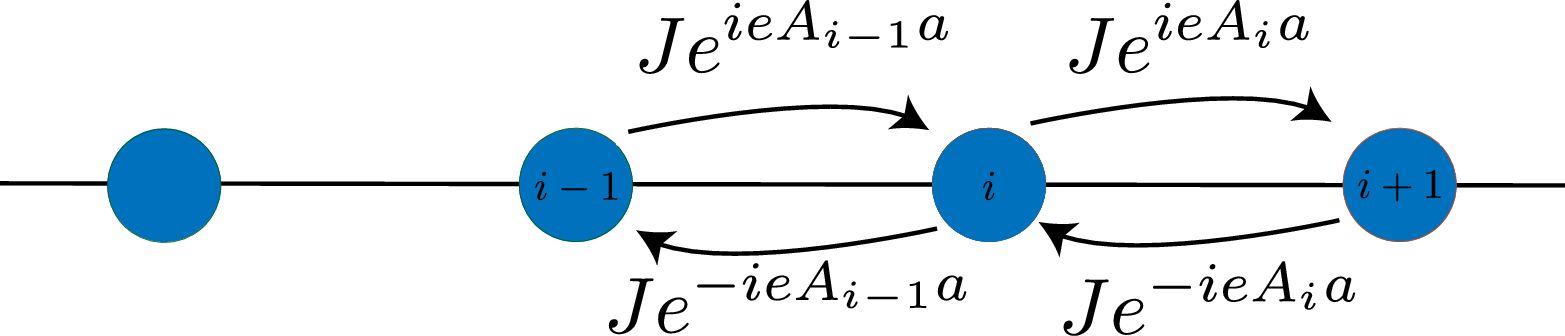
\includegraphics[width=0.70\columnwidth]{figures/SimpleHopping/SimpleHoppingv2}
\caption{{Hopping in the lattice after a U(1) gauge transformation. At each
hopping event to right, the particle acquires a phase
\(e\ A_i\ a\), which is proportional to the vector potential.
Hopping to the left leads to the accumulation of the inverse phase
\(-e\ A_ia\).
{\label{840410}}%
}}
\end{center}
\end{figure}


 \subsection{From the gauge symmetry to particle conservation}
 We have seen that the equations of motion remain the same if the wave function is multiplied by a phase that is constant in space and time. We can see this directly from Eq. \eqref{Eq:LatticeWithMagField} with $\varphi_j(t) = \varphi$.
 So we obtain:
 \begin{eqnarray}
 U_C &= e^{i\varphi\sum_j\hat{N}_j }\\
 \tilde{H} &= UHU^\dag  = H\\
 \Rightarrow UH &= HU\\
 \Rightarrow [H,U] &= 0
 \end{eqnarray}
 If the unitary operator commutes with the Hamiltonian, we also now that its generator $\hat{N} = \sum_j\hat{N}_j$ commutes:
 \begin{align}
 [H,\hat{N}] =0
 \end{align}
 And as the number generator does not depend explicitly on time we obtain from the Heisenberg equation that the total number of atoms is conserved.


 \section{The Wilson approach to dynamical gauge fields}\label{Sec:Wilson}
 Until now we seen that there is an intimate relation between the existance of electric and magnetic fields and $U(1)$ gauge transformations that depend on time and position. However, the gauge fields are not changing in any way as we are moving a charge. This is in direct constrast to electrodynamics where the motion of the charge implies directly the change of the electric field, see Fig. \ref{333433}. This relationship is captured by Gauss' Law:
 \begin{equation}\label{Eq:GaussLaw}
 \mathbf{div} \mathbf{E} = \rho
 \end{equation}
 
 Further the time evolution of the vector potential  is not at all captured in the previous section. In electrodynamics we actually have to fulfill the relation:
 \begin{equation}\label{Eq:MaxwellTime}
 \partial_t \mathbf{A} = \mathbf{E}
 \end{equation}\selectlanguage{english}
\begin{figure}[h!]
\begin{center}
\includegraphics[width=0.70\columnwidth]{figures/output-wsBM9r/output-wsBM9r}
\caption{{Gauss law of electrodynamics. As the charge (blue) is displacted, the
electric fiel is also modified. This perfect correlation between
electric field and matter field, is one of the cornerstones of any
realization of dynamical gauge fields in synthetic systems.
{\label{333433}}%
}}
\end{center}
\end{figure}

 
 To implement these two constraint, we will have to modify the underlying Hamiltonian. So we look once again at the Hamiltonian \eqref{Eq:LatticeWithMagField} and rewrite it in a more suggestive way:
 \begin{equation}\label{eq:LatticeWithLink}
 \tilde{H} = -J\sum_i \left[a_i^\dag L^*_i a_{i+1} +a_{i+1}^\dag L_i a_i - \dot{\varphi}_j \hat{N}_j\right]
 \end{equation}
  If the $L_i$ was an operator it would actually have a very similiar structure to the Gauss law. As the particle hops from site to site it would change the operator $L_i$. We will call them in the following the \textbf{link operators}. In the next section \ref{Sec:GaussLaw} , we adapt the Hamiltonian with dynamical links such that the system now fulfills Gauss' Law.  Then we will also add an additional term to the Hamiltonian to obtain the appropiate time dynamics of ED in Sec. \ref{Sec:TD}.



\subsection{Gauss law}\label{Sec:GaussLaw}
 Eq. \eqref{Eq:GaussLaw} describes a local conservation law combining the matter field and the electric field. So we will be able to obtain such a relation by enforcing local gauge symmetry. To derive the \textit{local} transformation laws, we will first perform a local gauge transformation of the matter field:
 \begin{eqnarray}
U =& e^{i\varphi_j \hat{N}_j}\\
\tilde{H} =&-J\sum_{i\neq j, j-1}\left[a_i^\dag \hat{L}^\dag_i a_{i+1} +a_{i+1}^\dag \hat{L}_i a_i\right]\\
  &- J \left[a_{j-1}^\dag \hat{L}^\dag_{j-1} a_{j} e^{i\varphi_j} +a_{j}^\dag \hat{L}_{j-1}a_{j-1} e^{-i \varphi_j}\right]  \nonumber\\
  &- J \left[a_{j}^\dag \hat{L}^\dag_{j} a_{j+1} e^{-i\varphi_j} +a_{j+1}^\dag \hat{L}_{j}a_{j} e^{i \varphi_j} - \dot{\varphi}_{j}\hat{N}_j\right]  \nonumber
\end{eqnarray}
 So we would obtain local gauge symmetry if we find a transformation of the form:
 \begin{eqnarray}
 ~\tilde{L}_j &= L_j e^{-i\varphi_j}\\
 ~\tilde{L}_{j-1} &= L_{j-1} e^{i\varphi_j}
 \end{eqnarray}
 This gauge transformation enforces the following conditions on the generator of the gauge transformation:
 \begin{align}
\exp(i\varphi G^L)L \exp(-i\varphi G^L) = \exp(-i\varphi)L
\end{align}
Let me write it in an infinitisimal way:
\begin{eqnarray}
\exp(i\varphi G^L)L \exp(-i\varphi G^L)  &= (1+i\varphi G^L)L (1-i\varphi G^L) \nonumber\\
&= (L+i\varphi G^L L) (1-i\varphi G^L)\nonumber\\
&= (L+i\varphi G^L L - i\varphi L G^L)\nonumber\\
&= (1-i\varphi )L\nonumber
\end{eqnarray}
We end up with:
\begin{equation}\label{Eq:CommLinkOps}
~[L,G^L] = L
\end{equation}

 So we can actually now know that the Hamiltonian remains unchanged under a gauge transformation with the generator  
  \begin{eqnarray}
G_j &= \hat{N}_j + G^L_j - G^L_{j-1}\\
 \tilde{H} =& -J\sum_{i}\left[a_i^\dag \hat{L}^\dag_i a_{i+1} +a_{i+1}^\dag \hat{L}_i a_i\right]- J \dot{\varphi}_{j}\hat{G}_j 
\end{eqnarray}

So if we want to have gauge symmetry even for time dependent gauge transformations we have to fulfill
\begin{align}
\hat{G}_j\ket{\psi} = 0
\end{align}
Additionally we can take a closer look at the structure of the generator, which can actuall rewrite as something similiar to Gauss' law:
\begin{eqnarray}
\hat{G}_j &= \hat{N}_j + G^L_j - G^L_{j-1} \\
&= \hat{N}_j + (\mathbf{div}G^L)_j\\
&= \hat{N}_j + \frac{1}{\ch}(\mathbf{div}E)_j
\end{eqnarray}
So we know that the electric field is basically the generator of the local gauge transformation of the link operators. Using Eq. \eqref{Eq:CommLinkOps} we can write down the commutation relation between link operator and electric field as:
\begin{equation}
~[L_i,E_i] = \ch L_i
\end{equation}
However, we do not know the value of the charge, nor the commutation relations of the link operators. We will obtain them from the time evolution of the gauge field.

\subsection{Time dynamics}\label{Sec:TD}
 
 In analogy with classical mechanics we can introduce the Hamiltonian dynamics of the electric field via an $E^2$ term. So the full Hamiltonian reads now:
 \begin{equation}
  H = \chi_L \sum_i (G^L_i)^2 - J\sum_i \left[a_i^\dag L^\dag_i a_{i+1} +a_{i+1}^\dag \hat{L}_i a_i \right]
 \end{equation}
We now have to look at the time dynamics of the link operators. We obtain:
\begin{equation}
i\dot{L}_j = \chi_L [(G^L_j)^2,L_j] - J\sum_i \left[a_i^\dag [L^\dag_i,L_j] a_{i+1} +a_{i+1}^\dag [\hat{L}_i,L_j] a_i \right]\nonumber
\end{equation}
Comparing to Eq. \eqref{Eq:MaxwellTime} we see that the commutators between the links should disappear. So we should enforce:
\begin{eqnarray}
 [L^\dag_i,L_j]  &= 0\\
 ~[L_i,L_j]  &= 0\\
 ~[L^\dag_i,L^\dag_j]  &= 0
\end{eqnarray}
At this stage we know that the link operators are unitary:
\begin{align}
L_i^\dag L_i = L_i L_i^\dag
\end{align}
So in analogy with the classical case we will identify its phase with the vector potential as:
\begin{align}
L_i = e^{i\ch A_i \aL}
\end{align}
Let us now continue to look into the time evolution.
\begin{eqnarray}
i\dot{L}_j &= \chi_L [(G^L_j)^2,L_j] \\
&=\chi_L \left(G^L_j[G^L_j,L_j]+[G^L_j,L_j]G^L_j\right)\\
&= -\chi_L \left(G^L_jL_j+L_jG^L_j\right)
\end{eqnarray}
And in the classical limit we find now:
\begin{equation}
-\ch \aL \dot{A}_j = -2\chi_L  \frac{E_j}{\ch}
\end{equation}
 So we know now that:
\begin{align}
 \chi_L= \frac{\ch^2 \aL}{2}
\end{align}
Our Hamiltonian reads therefore:
\begin{equation}
H = \frac{\aL}{2} \sum_i E_i^2 + \frac{1}{2m a_L^2}\sum_i \left[a_i^\dag L^\dag_i a_{i+1} +a_{i+1}^\dag \hat{L}_i a_i \right]
\end{equation}
End then we can identify
\footnote{What do we learn from that ? Does the theorist agree ?}:
\begin{eqnarray}
\chi_L= \frac{\ch^2 \aL}{2}\\
J= \frac{1}{2ma_L^2}
\end{eqnarray}

\section{The quantum link approach to dynamical gauge fields}\label{Sec:QLM}
 
 The previous approach relies on unitary link operatores, which are extremely hard to implement with ultracold atomic gases. The idea of QLM is relax the constraints on the link operators a bit, while keeping exactly the local gauge invariance. This is also the only formalism for which proposals of analog quantum simulation exist as discussed in Ref. \cite{Wiese2013,Zohar2016,Kasper_2016,Kasper_2017} and citations therein. The discussion on the Gauss' law remains the same as in the previous section, so we would like to have:
 \begin{equation}\label{eq:CommutRelLinks}
[L_i,G^L_i] = L_i ~~[L^\dag_i,G^L_i] = -L^\dag_i
\end{equation}




\subsection{Using spins as links}
 
A nice way out of the problems with finding a unitary link operator was suggested by \cite{Chandrasekharan1997,Horn1981,Orland1990}. 
Actually, we can decompose the link into its real and imaginary part: 
 \begin{equation}\label{Eq:LatticeWithLink}
 L_i = e^{i\ch A_i \aL} =\cos(\ch A_i \aL) + i\sin(\ch A_i \aL)
 \end{equation}
 Instead of using a cosine function we now simply set the real and imaginary part as operators:
  \begin{eqnarray}
 \hat{L}_i = \hat{C}_i + i\hat{S}_i\\
 \hat{L}_i^\dag = \hat{C}_i - i\hat{S}_i
 \end{eqnarray}
 We can now plug in these definitions into equation \eqref{eq:CommutRelLinks} and obtain:
 \begin{eqnarray}
[C + i S,G] &= C + iS \\
~[C,G] + i [S,G] &= C + iS \\
~[C,G] &= iS \label{Eq:CommSpinLinks}
\end{eqnarray}
In a similiar fashion we have:

\begin{eqnarray}
[C - i S,G] = -(C - iS)\\
~[C,G] - i [S,G] = iS -C\nonumber\\
~[G,S] = iC\label{Eq:CommSpinLinks}
\end{eqnarray}
The last line sets the commutation relationship of the links. These can be directly identified with the commutation relationships of a spin. 
So we directly find that we will be able to represent the link operator by composition of spins:
\begin{eqnarray}
C = J_x\\
S = J_y\\
G = -J_z
\end{eqnarray}
And we can also write down the link operator as:
\begin{eqnarray}
L &= J_x + iJ_y = J_+\\
L^\dag &=J_x - iJ_y = J_-
\end{eqnarray}
Let us write down explicitly once more the commutation relationships that we have in the QLM:
\begin{equation}
[L_i, G^L_i]=[J_+, -J_z] =J_+\label{eq:CommLinkQLM}
\end{equation}

So while we keep local gauge invariance, we have now non-commutating link operators. This means that we implement properly the Gauss' law. However, the time evolution will only correspond in certain limits to the time evolution of QED. As reminder each operator acts in the following way on an eigenstate:
\begin{eqnarray}
J^2 \ket{m,\ell}&= \ell(\ell+1)\ket{m,\ell}\\
J_z \ket{m,\ell}&= m\ket{m,\ell}\\
J_+\ket{m,\ell} &=\sqrt{\ell(\ell+1)-m(m+1)}\ket{m+1,\ell}\\
J_-\ket{m,\ell} &=\sqrt{\ell(\ell+1)-m(m-1)}\ket{m-1,\ell}
\end{eqnarray}

\subsection{Identification with QED}

We can once again write down our microscopic Hamiltonian:
\begin{equation}
H_{QL} = \chi_L \sum_i (J_z^i)^2-J\sum_i \left[a_i^\dag \hat{J}^+_i a_{i+1} +a_{i+1}^\dag \hat{J}^-_i a_i \right]
\end{equation}
We would now like to make the connection to QED. For that we need the commutators in equation \eqref{eq:CommLinkQLM} to become negligable. 
 We actually know that this will typically happen in the limit of large occupation numbers for the spin. In this case we can write \href{http://www.kip.uni-heidelberg.de/Veroeffentlichungen/details.php?id=2160}{(PhD by Christian Gross)}:
\begin{eqnarray}
\hat{J}_x &\approx \ell \cos(\hat{\varphi})~~\hat{J}_y \approx \ell \sin(\hat{\varphi})\\
\Rightarrow J_+ &\approx \ell e^{i\hat{\varphi}}~~ J_- \approx \ell e^{-i\hat{\varphi}}
\end{eqnarray}
So we definitely want to take the prefactor $\ell$ out of hopping element and define:
\begin{align}
L_i^\dag = \frac{J_i^+}{\ell}~~L_i = \frac{J_i^-}{\ell}
\end{align}
So the Hamiltonian should now be written as:
\begin{equation}
H_{QL} = \chi_L \sum_i (J_z^i)^2+\frac{\ell}{m^* a_L^2}\sum_i \left[a_i^\dag \hat{L}^\dag_i a_{i+1} +a_{i+1}^\dag \hat{L}_i a_i \right]
\end{equation}

In the next step, we have to verify that the equations of motion are the appropiate ones. We obtain:
\begin{eqnarray}
i\dot{J}^+_i&=\chi_L [(J_z^i)^2, J_i^+]-Ja_{i+1}^\dag a_i [J_i^-,J_i^+]\\
&=-\chi_L (J_i^zJ_i^++J_i^+J_z^i)+2Ja_{i+1}^\dag a_i J^z_i
\end{eqnarray}
In the classical limit we obtain now:
\begin{eqnarray}
-\ell \ch\dot{A}_i \aL=  \left(\frac{-2\chi_L \ell}{\ch}+2Ja_{i+1}^\dag a_i\right)E_i\\
\dot{A}_i=  \left(\frac{2\chi_L }{\ch^2\aL}-\frac{2Ja_{i+1}^\dag a_i}{\ch\ell\aL}\right)E_i
\end{eqnarray}
So the coherence could now be driving the dynamics as in the usual spin changing collision. However, let us simply assume that it is in the order of one. Then obtain the condition for finding the QED limit that:
\begin{eqnarray}
\frac{2\chi_L }{\ch^2\aL}&\gg\frac{2J}{\ch\ell\aL}\\
\ell&\gg\frac{J\ch}{\chi_L}
\end{eqnarray}
If we have this condition we can actually write down once again the previous equation of motion, where we found that:
\begin{align}
\chi_L=\frac{\ch^2}{2\aL}
\end{align}

\section{From theory towards
experiments}\label{from-theory-towards-experiments}

The theoretical concepts of dynamical gauge fields in ultracold atomic
systems have been relatively well established in the last few years
CITATIONS and stuied in several theory groups. However, the experimental
efforts are still way behind the theoretical framework. The gap is
actually so strong that only a single experiment has been performed with
ultracold ions \cite{Martinez_2016}, which performed a digital quantum
simulation with \emph{four} qubits. With ultracold atomic gases,up to
the groups to decide on the specific experimental implementation, which
best implements the:

\begin{itemize}
\tightlist
\item
  Gauss law, which connects the matter field dynamics to the gauge field
  dynamics.
\item
  Time dynamics, which connects the vector potential dynamics to the
  electric field dynamics
\end{itemize}

And this is exactly, what we are working on in our
\href{https://www.kip.uni-heidelberg.de/synqs/dyngauge}{mixture lab} in
Heidelberg.

\selectlanguage{english}
\FloatBarrier
\bibliographystyle{plainnat}
\bibliography{bibliography/converted_to_latex.bib%
}

\end{document}

